\documentclass{config/apuntes}

\title{Análisis de Imagen Biomédica}
\author{Sandra Mingo Ramírez}
\date{2025/26}
\acronym{AIBM}

\usepackage[all]{nowidow}
\usepackage{listing}
\usepackage{color}
\usepackage{tabularx}
\usepackage{multirow}
\usepackage{makecell}
\usepackage{amsmath}
\usepackage{array}
\usepackage{soul}

\definecolor{dkgreen}{rgb}{0,0.6,0}
\definecolor{gray}{rgb}{0.5,0.5,0.5}
\definecolor{mauve}{rgb}{0.58,0,0.82}

\lstset{
  frame=tb,
  aboveskip=3mm,
  belowskip=3mm,
  showstringspaces=false,
  columns=flexible,
  basicstyle={\small\ttfamily},
  numbers=none,
  numberstyle=\tiny\color{gray},
  keywordstyle=\color{blue},
  commentstyle=\color{dkgreen},
  stringstyle=\color{mauve},
  breaklines=true,
  breakatwhitespace=true,
  tabsize=3
}

\usepackage{tocloft}

\advance\cftchapnumwidth 0.9em\relax
\advance\cftsecnumwidth 0.6em\relax
\advance\cftsubsecindent 0.5em\relax
\advance\cftsubsecnumwidth 0.5em\relax
\begin{document}

\begin{abstract}
En las ciencias biomédicas no solo se recogen datos; en ocasiones se generan imágenes que posteriormente se deben analizar y de las que se debe extraer información comprensiva. 
El análisis de imagen biomédica es el proceso de examinar y extraer información útil de imágenes biomédicas, como resonancias magnéticas, tomografías computarizadas (TC) o ecografías, para facilitar diagnósticos, monitorear el progreso de enfermedades y desarrollar nuevas técnicas de diagnóstico y tratamiento. El prefijo "bio" se refiere a la fase preclínica, siendo así las imágenes de modelos animales fundamentalmente.
\end{abstract}

\pagestyle{plain}

\maketitle

\tableofcontents

%2 profesores y 2 invitados
%3 aplicaciones: microscopía, PET y resonancia magnética
% 60 % examen -> convocatoria en enero,
% 15 % Moodle
% 25 % pequeños trabajos

% Programación en Matlab - versión gratuita para estudiantes, 
% Octave alternativa gratuita a Matlab

%16/09 - Blanca Lizarbe
\chapter{Introducción al procesado de imágenes}
\section{Formación de imágenes}
Hay muchas formas de obtener una imagen, dependiendo de la fuente de energía (p. ej., fotones, ondas de radio, ultrasonido) y del sistema detector que la capture. Los tipos de imágenes se clasifican según si la formación es directa o indirecta, analógica (continua) o digital, y según el tipo de energía utilizada (radiación electromagnética, acústica, etc.).

Una forma de clasificarlas es en función del tipo de energía o radiación utilizada. La luz visible es una pequeña parte del espectro electromagnético. Las imágenes biomédicas pueden generarse utilizando otras partes de este espectro (rayos X, radiofrecuencia), así como otras formas de energía como ondas mecánicas (sonar, ultrasonido) o campos (magnéticos, eléctricos).

Aunque el grueso del curso sea el análisis y procesado de las imágenes, es importante saber de dónde vienen y su contexto.
\begin{itemize}
\item La \textbf{formación de imagen de rayos X} proviene de una fuente emisora. Estos rayos interaccionan con el tejido biológico (son atenuados principalmente por absorción y dispersión). La radiación que atraviesa el tejido incide sobre un detector (que históricamente era una placa fotográfica o de película, pero hoy son casi exclusivamente detectores digitales como placas de fósforo o detectores planos).
\item La \textbf{formación de una imagen de Resonancia Magnética (RM)} se basa en aplicar un campo magnético estático y fuerte (B0) al tejido, alineando los momentos magnéticos de los núcleos de hidrógeno. Se aplican pulsos de radiofrecuencia (RF) para excitar estos núcleos, que al relajarse emiten señales de RF. Esta señal se detecta con bobinas. Utilizando gradientes de campo magnético (que varían el campo de forma lineal en el espacio), se puede codificar espacialmente la señal y reconstruirla digitalmente para asignar diferentes intensidades de señal a cada voxel (elemento de volumen 3D) o píxel (2D).
\end{itemize}

\subsection{De analógico a digital}
Para convertir una imagen analógica (como una placa de rayos X o una fotografía) a digital se utiliza un dispositivo de digitalización, como un escáner o un detector digital directamente. Este proceso implica \textbf{muestrear (sampling)} la imagen, dividiendo el espacio en una matriz discreta de elementos (píxeles), y \textbf{cuantizar} la intensidad de luz en cada punto, asignándole un valor digital discreto.

La resolución espacial tiene que ver con el nivel de detalle discernible, determinado por el tamaño del píxel y las propiedades del sistema de imagen. Una imagen con muchos píxeles pequeños (alta resolución) permite visualizar detalles finos y bordes definidos. En cambio, una imagen de baja resolución tiene pocos píxeles grandes, lo que resulta en una pérdida de detalles y una apariencia pixelada o borrosa al ampliarla.

Las imágenes con las que se suele trabajar en diagnóstico por imagen suelen representarse en escala de grises. Esto significa que a cada píxel se le asigna una intensidad lumínica representada por un valor numérico. En el formato estándar de 8 bits, este valor va de 0 (negro) a 255 (blanco), permitiendo $2^8 = 256$ tonos de gris intermedios. La cantidad de bits utilizada para representar el valor de un píxel se denomina profundidad de bits (bit depth).
%Importante el concepto de 256 niveles de gris y los 8 bits

Cualquier sistema moderno de formación de imagen biomédica integra \textbf{sensores} (o detectores) y un \textbf{conversor de analógico a digital (ADC).} La imagen digital se debe guardar, procesar y, en ocasiones, se reconvierte a analógico (por ejemplo, mediante una pantalla) para su visualización.

\section{Procesado de imágenes digitales}
Dentro del procesamiento de imagen hay varias categorías o pasos:
\begin{enumerate}
\item \textbf{Mejora o Realce de la Imagen (Image Enhancement):} Técnicas para ajustar propiedades como el brillo, el contraste o para aplicar filtros (como la convolución) con el fin de hacer ciertas características más visibles para el observador humano o para un algoritmo posterior. Incluye la corrección de algunos artefactos.
\item \textbf{Restauración de Imagen (Image Restoration):} Su objetivo es eliminar o reducir la degradación (como el desenfoque o el ruido) utilizando un modelo de cómo se degradó la imagen. Se busca aproximarse a la imagen original no degradada.
\item \textbf{Análisis de la Imagen (Image Analysis):} Procesos como la segmentación (delimitación de regiones de interés), la extracción de características (cálculo de métricas cuantitativas) y la clasificación de objetos.
\item \textbf{Compresión de Imagen (Image Compression):} Técnicas para reducir el tamaño de los archivos de imagen para su almacenamiento o transmisión eficiente (p. ej., JPEG, JPEG 2000, DICOM con compresión).
\item \textbf{Síntesis de Imagen (Image Synthesis):} Generación de imágenes a partir de modelos o datos, como en la reconstrucción tomográfica o la generación de imágenes mediante Inteligencia Artificial.
\end{enumerate}

\subsection{Image enhancement}
Las imágenes biomédicas se utilizan para el diagnóstico, tanto \textbf{cualitativo} (observación visual de morfología) como \textbf{cuantitativo} (medición de parámetros fisiológicos o bioquímicos). Para el diagnóstico cualitativo, se tratan las imágenes para reducir ruido o realzar bordes. En las imágenes cuantitativas, el valor numérico del píxel tiene significado físico (p. ej., unidades Hounsfield en TC, concentración de un contraste, valores T1 o T2 en RM). Por ello, al manipular estas imágenes para su análisis, es crucial utilizar técnicas que no alteren o que corrijan de manera controlada los valores subyacentes, preservando la información biológico-física. A menudo, la consistencia en el procesamiento (aplicar el mismo algoritmo a todos los sujetos de un estudio) es más importante que la absolutez del valor.

Los \textbf{artefactos} son patrones o estructuras presentes en la imagen que no corresponden a la anatomía o fisiología real del sujeto, sino que son causados por el equipo, el protocolo de adquisición o el propio paciente. Estos incluyen desde artefactos por metal (implantes) hasta los causados por el movimiento voluntario o involuntario del paciente durante una adquisición, especialmente si es larga. La \textbf{reducción de ruido} (ruido aleatorio inherente a cualquier medición física) es también esencial para mejorar la relación señal-ruido (SNR).

Hoy día, las técnicas de \textbf{aprendizaje automático (machine learning),} y en particular las \textbf{redes neuronales convolucionales (CNN),} se utilizan extensamente. Un ejemplo es el entrenamiento de redes con pares de imágenes: una entrada degradada (p. ej., con artefactos de movimiento o ruido) y una salida objetivo de referencia ("ground truth") de alta calidad. La red aprende la transformación para mapear la imagen defectuosa a una versión corregida. Es importante destacar que a menudo el "ground truth" perfecto no existe \textit{in vivo}, por lo que los modelos se entrenan con datos simulados o con imágenes de alta calidad adquiridas en condiciones ideales.

Para corregir el ruido, una técnica común es el \textbf{filtrado espacial}. Un ejemplo básico es el \textbf{filtro Gaussiano}, que suaviza la imagen promediando los valores de los píxeles vecinos, ponderados por una función Gaussiana. Esto homogeniza las regiones y reduce el ruido, pero a costa de una potencial pérdida de detalle (suavizado de bordes). La operación se aplica deslizando un kernel (ventana) sobre la imagen, realizando una \textbf{convolución} (producto punto entre el kernel y los píxeles subyacentes) en cada posición.

\begin{figure}[h]
\centering
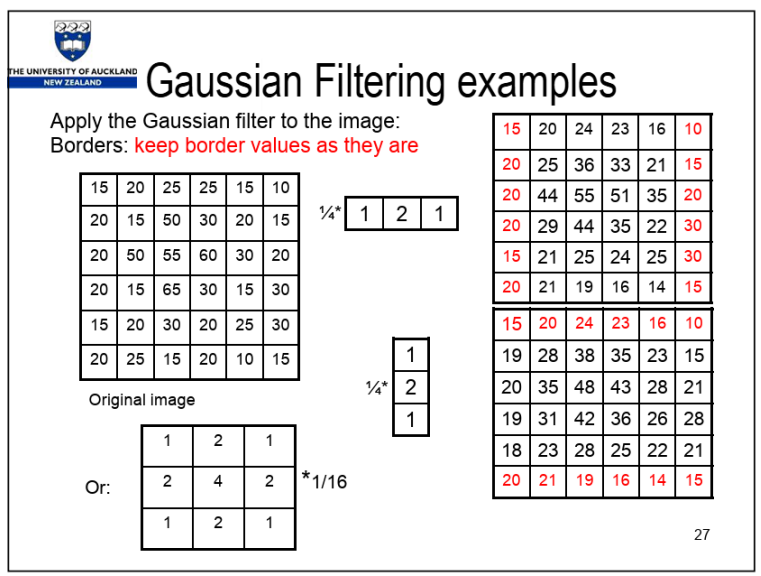
\includegraphics[width = 0.8\textwidth]{figs/gaussian-filter.png}
\caption{Ejemplo de filtro Gaussiano. Se aplica la matriz izquierda inferior sobre la imagen original, multiplicando los valores por la matriz de filtro y dividiendo por 16. Esto se realiza sobre cada píxel a excepción de los bordes. Por ejemplo, para el píxel con valor 15 de la segunda fila, segunda columna: $(15*1 + 20 * 2 + 25 * 1 + 20 * 2 + 15 * 4 + 50 * 2 + 20 * 1 + 50 * 2 + 55 * 1)/16 = 455/16 = 28,4375 \approx 28$, que es el valor del píxel de la matriz derecha inferior.}
\end{figure}

Mejora de la Resolución: El término general es superresolución (super-resolution). Este proceso busca estimar o reconstruir una imagen de alta resolución a partir de una o varias imágenes de baja resolución. El objetivo es recuperar detalles finos perdidos durante la adquisición, lo que conduce a una visualización más clara y puede facilitar un diagnóstico más preciso. Es importante distinguirlo de un simple zoom o interpolación, que agranda los píxeles sin añadir información nueva real. Las técnicas de superresolución pueden ser:
\begin{itemize}
\item \textbf{Basadas en reconstrucción:} Utilizan múltiples imágenes sub-píxel de la misma escena y algoritmos para fusionarlas.
\item \textbf{Basadas en aprendizaje:} Utilizan redes neuronales (como CNNs) entrenadas con pares de imágenes (baja/alta resolución) para aprender el mapeo que añade los detalles faltantes.
\end{itemize}

\subsection{Image analysis}
La \textbf{segmentación} es un paso fundamental en el análisis de imágenes. Su objetivo es dividir una imagen en regiones o estructuras significativas, permitiendo extraer y cuantificar la información de interés. Por ejemplo, aislar solo los huesos en una Tomografía Computarizada (TC), delimitar un tumor, o separar el ventrículo izquierdo en una imagen cardiaca.

Se lleva a cabo mediante algoritmos que identifican boundaries (bordes) o regiones homogéneas basándose en propiedades como la intensidad, el color, la textura o el contexto. No se limita solo a la extracción de bordes; existen múltiples enfoques:
\begin{itemize}
\item Basados en umbral (thresholding): Separan según el valor de intensidad.
\item Basados en regiones (region growing, watershed): Agrupan píxeles conectados con propiedades similares.
\item Basados en bordes (edge detection): Identifican discontinuidades en la intensidad (usando operadores como Sobel, Canny).
\item Basados en modelos (active contours, level sets): Utilizan curvas o superficies que evolucionan para ajustarse a los contornos.
\item Basados en aprendizaje (Machine/Deep Learning): Las redes neuronales (especialmente las U-Net) aprenden a segmentar a partir de ejemplos etiquetados.
\end{itemize}

El \textbf{registro de imágenes (Image Registration)} es el proceso de alinear geométricamente dos o más conjuntos de imágenes (datasets) adquiridas en diferentes momentos, desde diferentes modalidades o desde distintos puntos de vista. El objetivo es establecer una correspondencia punto a punto entre ellas para poder comparar, fusionar o analizar la información de forma coherente.

Esto se logra encontrando la transformación espacial óptima que mapea los puntos de una imagen (imagen móvil o "moving") sobre los de otra (imagen de referencia o "fixed"). Los tipos de transformación, ordenados de menor a mayor complejidad y flexibilidad, son:
\begin{itemize}
\item \textbf{Registro rígido (Rigid):} Alinea imágenes solo con rotaciones y traslaciones (desplazamientos) globales. Preserva las distancias y ángulos entre todos los puntos. Es útil para imágenes de la misma anatomía sin cambios internos (p. ej., cabeza en diferentes estudios de RM).
\item \textbf{Registro por similitud (Similarity):} Añade escalado isotrópico (mismo factor de escala en todos los ejes) a la transformación rígida. Preserva las formas y los ángulos, pero no las distancias absolutas.
\item \textbf{Registro afín (Affine):} Incluye cizallamiento (shearing) y escalado anisotrópico (diferente factor en cada eje), además de las transformaciones rígidas y de escalado. Las líneas paralelas siguen siéndolo después de la transformación, pero los ángulos pueden no conservarse. Es útil para corregir diferencias de adquisición o geometría entre modalidades.
\item \textbf{Registro no rígido o deformable (Non-rigid/Deformable):} Maneja deformaciones elásticas o fluidas complejas, localizadas y no lineales. Es esencial para compensar movimientos de órganos (como el corazón o los pulmones), cambios anatómicos (crecimiento de un tumor) o para alinear imágenes de pacientes diferentes en un atlas poblacional.
\end{itemize}

%17/09 - Álvaro García
\chapter{Fundamentos imagen biomédica}
\section{Percepción visual}
\subsection{Fenómeno de la luz}
Una fuente de luz \textbf{monocromática} emite radiación predominantemente en una única \textbf{longitud de onda} (o frecuencia), percibida como un color puro. Un ejemplo característico es el láser. Por el contrario, la luz \textbf{policromática} está compuesta por una mezcla de múltiples longitudes de onda, como la luz solar o la de una bombilla LED blanca.

Existen dos tipos de fuentes luminosas:
\begin{itemize}
\item \textbf{Fuentes Primarias o Emisivas:} Generan su propia luz mediante procesos de excitación de átomos o moléculas (ej.: el Sol, una bombilla, un LED).
\item \textbf{Fuentes Secundarias o Reflectantes:} No generan luz propia, sino que reflejan total o parcialmente la luz que reciben de una fuente primaria (ej.: la Luna, un libro, la mayoría de los objetos que nos rodean). Casi todo lo que vemos son fuentes secundarias.
\end{itemize}

\subsection{Sistema visual humano}
El proceso de la visión comienza cuando la luz entra en el ojo y es proyectada sobre la \textbf{retina}, donde los \textbf{fotorreceptores} la captan y la convierten en señales electroquímicas (proceso de \textbf{transducción}). Estas señales se transmiten a través del \textbf{nervio óptico} al cerebro, donde se interpretan para generar la percepción visual.

Desde un punto de vista óptico, el ojo humano es análogo a una cámara fotográfica:
\begin{itemize}
\item \textbf{Lente:} El cristalino (junto con la córnea y los humores acuoso y vítreo) se encarga de enfocar la luz, proyectando una imagen nítida sobre la retina. Su forma se ajusta en un proceso llamado acomodación.
\item \textbf{Diafragma}: El iris (la parte coloreada) actúa como un diafragma, controlando el tamaño de la pupila para regular la cantidad de luz que entra en el ojo.
\item \textbf{Sensor}: La retina equivale al sensor de una cámara (CCD/CMOS). Es una capa de tejido sensible a la luz ubicada en la parte posterior del ojo.
\end{itemize}

La retina contiene dos tipos principales de fotorreceptores:
\begin{itemize}
\item \textbf{Bastones}: Altamente sensibles a la intensidad lumínica (luminancia), pero no al color. Son responsables de la visión escotópica (visión en condiciones de baja iluminación). Se concentran en la periferia de la retina, siendo muy sensibles al movimiento.
\item \textbf{Conos}: Menos sensibles que los bastones, pero especializados en la percepción del color (visión fotópica, en condiciones de alta iluminación). Se concentran en la fóvea, la zona central de la retina de máxima agudeza visual. Existen tres tipos, cada uno con un pico de sensibilidad a diferentes longitudes de onda: rojo (larga), verde (media) y azul (corta).
\end{itemize}

La capacidad del ojo tiene limitaciones físicas. La \textbf{resolución espacial} (capacidad para discernir detalles finos) y la \textbf{resolución temporal} (capacidad para discernir eventos rápidos) son finitas debido al número limitado de fotorreceptores y a su tiempo de respuesta.

La \textbf{agudeza visual} es la capacidad de distinguir entre dos puntos separados. Si la separación angular entre ellos es superior a \textbf{1 minuto de arco} (1/60 de grado), estimulan fotorreceptores y fibras nerviosas diferentes, por lo que el cerebro los percibe como entidades distintas. Si la separación es menor, ambos puntos estimulan el mismo receptor, y el cerebro percibe una \textbf{mezcla aditiva espacial (MAE)}, fusionándolos en un solo estímulo de color.

\begin{figure}[h]
\centering
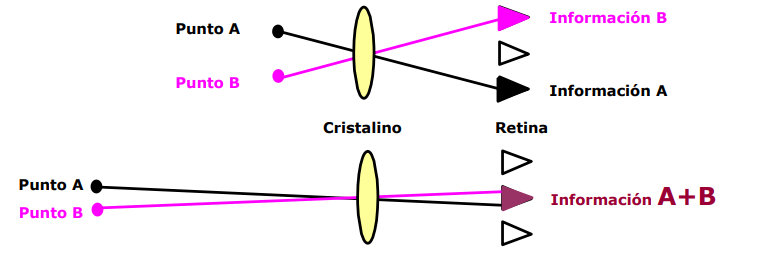
\includegraphics[width = \textwidth]{figs/mae.png}
\caption{Ilustración del principio de la mezcla aditiva espacial. Puntos de color suficientemente pequeños y cercanos se perciben como un color uniforme.}
\end{figure}

Este principio es fundamental en tecnologías de visualización como las pantallas de televisión y monitores, donde la imagen se forma mediante \textbf{píxeles} compuestos por subpíxeles rojos, verdes y azules (triadas de colores) cuya separación es inferior al umbral de agudeza visual.

La \textbf{memoria visual} o persistencia retiniana es una propiedad por la cual la excitación de los fotorreceptores no cesa instantáneamente tras desaparecer el estímulo, sino que continúa enviando señales al cerebro durante un breve periodo. La integración de impulsos luminosos consecutivos da lugar a la sensación de continuidad, un fenómeno conocido como \textbf{mezcla aditiva temporal (MAT)} o persistencia retiniana.

\begin{figure}[h]
\centering
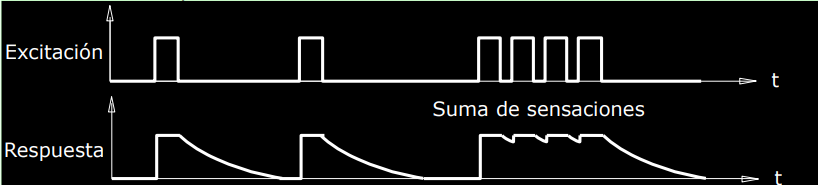
\includegraphics[width = \textwidth]{figs/mat.png}
\caption{Ilustración del principio de la mezcla aditiva temporal. Estímulos discretos sucesivos se perciben como un continuo si la frecuencia es suficientemente alta.}
\end{figure}

Si el intervalo entre impulsos es mayor de aproximadamente 40-50 ms (equivalente a 20-25 Hz), se percibe un parpadeo o \textit{flicker} molesto. Por debajo de este umbral, la respuesta al nuevo estímulo se suma a la anterior, creando una sensación de flujo continuo. Esto explica por qué una secuencia de imágenes estáticas (fotogramas) a una velocidad superior a 25 fps (fotogramas por segundo) se percibe como movimiento continuo. El umbral exacto varía con la luminancia y el campo visual estimulado.

\subsection{Luz}
La visión de los objetos no emisivos se debe a la reflexión (y en algunos casos, a la transmisión) de la luz que incide sobre ellos. La intensidad de la luz reflejada ($L$, luminancia) que llega al ojo depende de la intensidad de la luz incidente ($E$, iluminancia, medida en lux) y de las propiedades reflectivas del material ($R$).

En términos generales, se puede modelar como:
$$C_R(X, V, geom, t, \lambda) = E(X, t, \lambda).r(V, geom, \lambda)$$

Donde:
$R(V, \text{geom}, \lambda)$ es la reflectancia del material, que depende del ángulo de visión ($V$), la geometría de la superficie (si es rugosa/difusa o lisa/especular) y la longitud de onda ($\lambda$). Un objeto parece de un color porque absorbe selectivamente ciertas longitudes de onda y refleja otras.

Existen dos modelos de síntesis de color:
\begin{itemize}
\item \textbf{Síntesis Aditiva}: Propia de las fuentes de luz primarias. Los colores se crean sumando diferentes longitudes de onda de luz. La suma de los colores primarios aditivos (Rojo, Verde, Azul - RGB) en su máxima intensidad produce la percepción de blanco. Ej.: pantallas, monitores.
\item \textbf{Síntesis Sustractiva}: Propia de los pigmentos y materiales (fuentes secundarias). Los colores se crean porque el material absorbe (sustrae) ciertas longitudes de onda de la luz blanca incidente y refleja otras. Los colores primarios sustractivos son Cian, Magenta y Amarillo (CMY). La "suma" teórica de los tres absorbería toda la luz, produciendo negro. Ej.: pintura, impresión.
\end{itemize}

\subsection{Percepción de luminancia y color}
El sistema visual humano opera en tres regímenes de visión según el nivel de iluminación:
\begin{itemize}
\item \textbf{Visión Escotópica}: Activada en condiciones de muy baja iluminación (noche). Dominada por los bastones. No permite la percepción del color (visión en escala de grises) y tiene una baja agudeza visual.
\item \textbf{Visión Fotópica}: Activada en condiciones de alta iluminación (día). Dominada por los conos. Permite la percepción del color y una alta agudeza visual.
\item \textbf{Visión Mesópica}: Régimen intermedio (amanecer, atardecer, iluminación tenue). Participan tanto bastones como conos. La percepción del color y la agudeza visual son intermedias.
Los colores y nuestros conos no son puros. Los conos verdes absorben más que los conos rojos y azules. Nuestro cerebro recibe la información de los tres sensores y los integra para percibir un color u otro. 
\end{itemize}

La respuesta espectral de los tres tipos de conos se solapa. El cerebro deduce el color percibido (\textbf{crominancia}) a partir de la \textbf{señal tricromática} comparada que envían estos tres tipos de receptores. La crominancia se describe mediante dos atributos:
\begin{itemize}
\item \textbf{Tono:} el color en sí mismo.
\item \textbf{Saturación:} la pureza o intensidad del color.
\end{itemize}

Por otro lado, la \textbf{luminancia} se refiere a la cantidad de luz medida físicamente (en candelas/$m^2$), que se percibe subjetivamente como \textbf{brillo} en una escala de grises.


\begin{figure}[h]
\centering
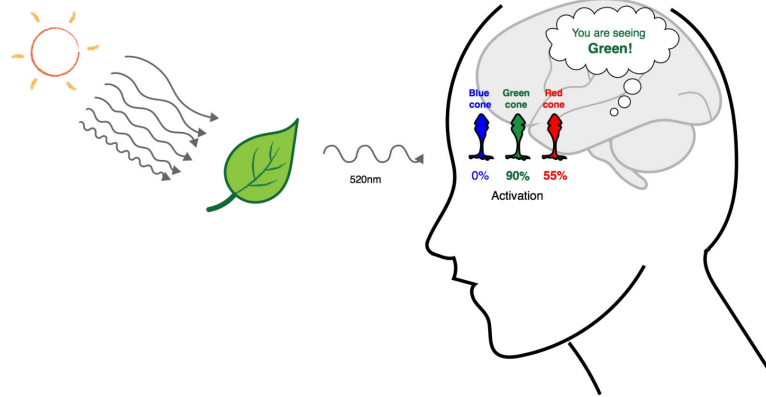
\includegraphics[width = \textwidth]{figs/perception.png}
\caption{Representación de la percepción visual, desglosando la información en componentes de luminancia (brillo) y crominancia (tono y saturación).}
\end{figure}

\subsection{Brillo}
El brillo es la percepción subjetiva de la luminancia. El sistema visual es extraordinariamente adaptable, capaz de funcionar en un rango de aproximadamente $10^{10}$ niveles de intensidad lumínica mediante el proceso de adaptación (ajuste de la sensibilidad retinal según la luminancia media del entorno).

La percepción del brillo es relativa, no absoluta. Depende críticamente del contraste entre un objeto y su fondo o entorno inmediato (Ley de Weber-Fechner). El ojo es mucho más sensible a las variaciones de luminancia (bordes, movimientos) que a los valores constantes.

No existe una medida física directa del brillo, ya que es una experiencia perceptiva compleja. En condiciones de alta luminancia (visión fotópica), el ojo tiene una mayor agudeza para discernir objetos claros sobre fondos oscuros. En condiciones de baja luminancia (visión escotópica o mesópica), la sensibilidad cambia, y puede resultar más fácil discernir objetos de luminancia media. 

Dado que la percepción del brillo es relativa, su evaluación debe considerar necesariamente el entorno. La \textbf{evaluación del contraste} es, por tanto, la medición cuantitativa de la diferencia percibida en luminancia (brillo) entre un objeto de interés (por ejemplo, un texto) y su fondo inmediato. Esta diferencia se expresa comúnmente como una razón de contraste (por ejemplo, 4:1, 7:1), que se calcula dividiendo la luminancia relativa de la parte más clara entre la de la parte más oscura. Un contraste alto asegura que la información sea discernible para el sistema visual, lo que es un principio crítico en disciplinas como el diseño de interfaces, la señalética y la accesibilidad web, garantizando que el contenido sea legible para usuarios con diversas capacidades visuales o en condiciones de iluminación variables.

\section{Captura de imágenes}
\subsection{Sistema de adquisición}
Los elementos funcionales fundamentales de un sistema de adquisición de imágenes son: el \textbf{sistema óptico} (o grupo óptico), el \textbf{sensor de imagen} (con sus distintas tecnologías y características) y la etapa de \textbf{procesamiento de la señal} (que convierte la información cruda del sensor en una imagen o señal de vídeo utilizable).

En una cámara, la exposición —la cantidad de luz que alcanza el sensor— se controla mediante dos mecanismos principales:
\begin{itemize}
\item El \textbf{obturador} controla la duración de la exposición (el intervalo de tiempo durante el cual la luz incide en el sensor).
\item El \textbf{diafragma} controla la intensidad de la luz que entra a través de la lente, ajustando el tamaño de la abertura.
\item El tercer elemento crucial es el propio \textbf{sensor}, compuesto por materiales fotosensibles (fotodiodos) que convierten la energía de los fotones (luz) en una señal eléctrica (carga).
\end{itemize}

\subsection{Modelo de cámara puntual \textit{pin hole}}
El modelo de cámara estenopeica o \textit{pinhole} es el modelo más simple de formación de imágenes. Sus componentes esenciales son:
\begin{itemize}
\item Un \textbf{centro de proyección} (el orificio estenopeico o \textit{pinhole}).
\item Una \textbf{distancia focal} ($f$), que es la distancia entre el centro de proyección y el plano de la imagen.
\item Un \textbf{plano de imagen} donde se forma la imagen proyectada.
\end{itemize}

Debido a la propagación rectilínea de la luz, la imagen formada en el plano es \textbf{invertida} (tanto vertical como horizontalmente). La principal ventaja de este modelo es que toda la escena está enfocada sin necesidad de un sistema de enfoque; la profundidad de campo es infinita.

Sin embargo, existe un compromiso (\textit{trade-off}) crítico en el tamaño del orificio:
\begin{itemize}
\item Si el orificio es demasiado grande, cada punto de la escena proyecta un pequeño círculo de confusión (\textit{circle of confusion}) en el plano de imagen, resultando en una imagen desenfocada debido a la superposición de estos círculos.
\item Si el orificio es demasiado pequeño, el fenómeno de la difracción de la luz se vuelve significativo. La luz se dispersa al pasar por la pequeña abertura, provocando que los puntos de la imagen se difuminen entre sí y se pierda definición y nitidez. Existe, por tanto, un tamaño de orificio óptimo que minimiza la combinación de estos dos efectos adversos.
\end{itemize}

\subsection{Color}
Los sensores de imagen (CCD o CMOS) son inherentemente \textbf{monocromáticos}; solo pueden medir la intensidad de la luz, no su longitud de onda (color). Para capturar imágenes en color, se emplean diversas estrategias que implican la separación de la luz en sus componentes espectrales:

\begin{itemize}
\item \textbf{Sistema de 3 Sensores (3-CCD/3-CMOS):} Utiliza un prisma dicroico para dividir la luz incidente en sus tres componentes espectrales primarias (rojo, verde y azul). Cada haz de color se dirige hacia un sensor dedicado. Este sistema ofrece la máxima calidad y fidelidad de color, ya que cada píxel de la imagen final se genera con información de intensidad completa para los tres canales. Su principal desventaja es el alto coste y la complejidad mecánica.
\item \textbf{Filtro de Color Rotativo:} Se coloca un filtro de color (rojo, verde o azul) giratorio delante de un único sensor. La cámara captura secuencialmente un fotograma para cada color primario. Este método es más económico que el de 3 sensores, pero introduce graves inconvenientes: baja calidad de color (especialmente con objetos en movimiento, que producen artefactos de \textit{ghosting}), una tasa de captura efectiva menor y la necesidad de una iluminación constante durante la rotación.
\item \textbf{Matriz de Filtros de Color (CFA - \textit{Color Filter Array}):} Es el método más común en cámaras consumer y profesionales. Consiste en un mosaico de microfiltros coloreados, depositado directamente sobre la superficie del sensor, donde cada filtro corresponde a un único fotodiodo (píxel). Cada píxel del sensor captura únicamente la intensidad de una componente de color (R, G o B). El patrón más utilizado es el filtro de Bayer (desarrollado por Bryce Bayer en Kodak, 1976), que utiliza un 50\% de filtros verdes, un 25\% de rojos y un 25\% de azules, imitando la mayor sensibilidad del ojo humano al verde.
\begin{figure}[h]
\centering
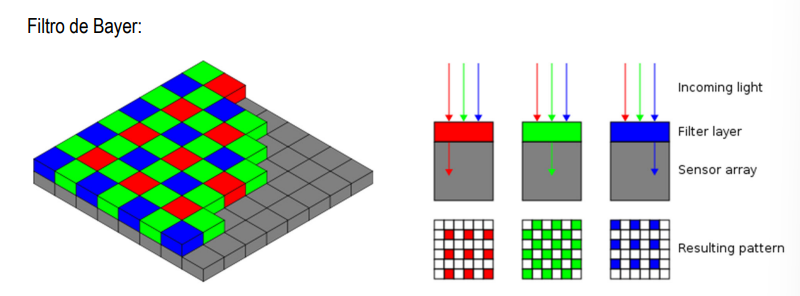
\includegraphics[width = \textwidth]{figs/filtro-bayer.png}
\end{figure}
La principal limitación de los CFA es que la resolución espacial de color es inferior a la resolución nominal del sensor. Para generar una imagen en color completa (donde cada píxel tenga valores R, G y B), es necesario aplicar un algoritmo de interpolación cromática o \textit{demosaicing}. Este proceso estima los componentes de color faltantes en cada píxel basándose en la información de los píxeles vecinos, lo que puede introducir artefactos como el \textit{moiré} o falseado de color (\textit{color aliasing}).
\end{itemize}

\section{Representación de imágenes}
\subsection{La imagen digital}
Una imagen digital es una representación bidimensional de una escena que ha sido \textbf{muestreada espacialmente y cuantificada en amplitud}. Esto significa que está definida en:
\begin{itemize}
\item Un dominio espacial discreto: un número finito de posiciones (píxeles) organizadas en una rejilla regular (matriz M×N).
\item Un rango de valores discreto: las intensidades solo pueden tomar un conjunto finito de valores (generalmente potencias de 2).
\end{itemize}

El \textbf{píxel} (elemento de imagen) es la unidad mínima de información espacial en una imagen digital. Cada píxel almacena un valor (o un conjunto de valores) que representa la intensidad luminosa y/o el color capturado por el sensor en esa posición específica. Así, una imagen digital puede representarse matemáticamente como una matriz de valores numéricos.

\subsection{True Color}
El término True Color se refiere a un método de representación de color que utiliza una codificación directa de los componentes cromáticos, típicamente capaz de representar más de 16 millones de colores distintos.

Es crucial hacer una distinción conceptual:
\begin{itemize}
\item \textbf{Imagen en Escala de Grises (Luminancia):} Se almacena un único valor por píxel, que representa la luminancia (la medida física de la intensidad de la luz), no la percepción subjetiva del brillo. Con una profundidad de 8 bits por píxel (bpp), se pueden representar 256 ($2^8$) niveles de gris, donde 0 suele representar el negro absoluto y 255 el blanco máximo.
\begin{figure}[h]
\centering
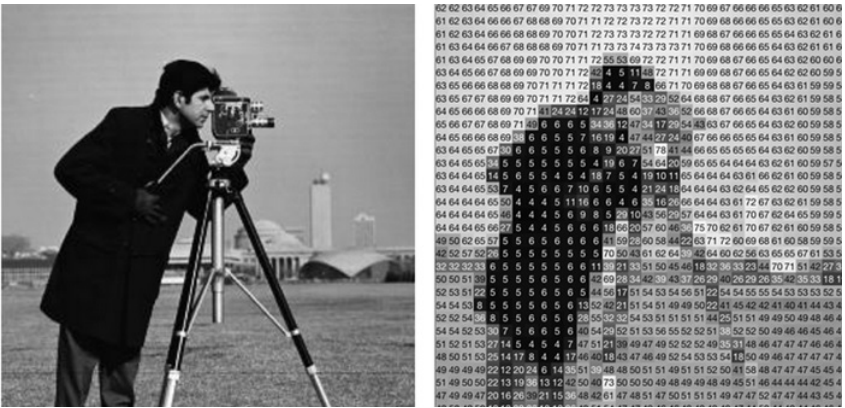
\includegraphics[width = 0.6\textwidth]{figs/true-color-mono.png}
\end{figure}

\item \textbf{Imagen True Color a Color}: Utiliza tres canales independientes (generalmente Rojo, Verde y Azul - RGB). Cada canal tiene una profundidad de 8 bits, resultando en un total de 24 bits por píxel (8 + 8 + 8). Esto permite representar $2^24 = 16.777.216$ colores distintos. Este tipo de imagen no es una matriz bidimensional simple, sino una estructura tridimensional de tamaño M×N×3, a menudo conceptualizada como "un cubo de información" donde cada "capa" corresponde a un canal de color.
\end{itemize}
\begin{figure}[h]
\centering
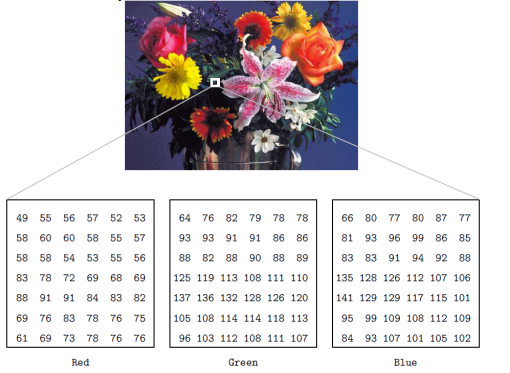
\includegraphics[width = 0.7\textwidth]{figs/true-color-tri.png}
\end{figure}

\subsection{Resolución vs definición}
La \textbf{resolución de la imagen (Pixel Dimensions}) se refiere al número absoluto de píxeles que componen la imagen en sus dimensiones de ancho y alto (e.g., 1920×1080 px). Es un atributo intrínseco del archivo digital y determina la cantidad de detalle espacial que la imagen contiene. El usuario puede seleccionarla durante la captura o el post-procesado (remuestreo).

La \textbf{Definición o Densidad de Píxeles (PPI - \textit{Pixels Per Inch} / DPI - \textit{Dots Per Inch})} es una medida de densidad que relaciona la resolución en píxeles con un tamaño físico real. Indica cuántos píxeles (PPI para pantallas) o puntos de tinta (DPI para impresión) hay en una pulgada lineal. Este valor define cómo de grandes o pequeños se verán los píxeles al reproducir la imagen en un dispositivo de salida (monitor, impresora). Está intrínsecamente ligado a la calidad del proceso de captura (óptica, sensor) y a las técnicas de procesamiento (interpolación, submuestreo) utilizadas.

\begin{figure}[h]
\centering
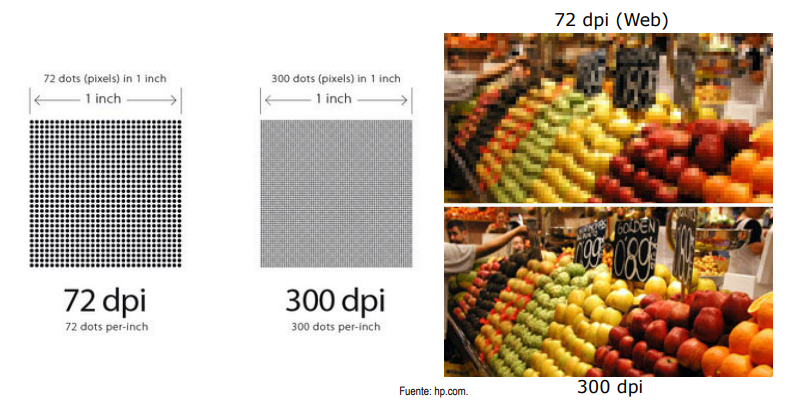
\includegraphics[width = 0.8\textwidth]{figs/resolucion-definicion.png}
\end{figure}

\subsection{Profundidad}
La profundidad de color se mide en bits por píxel (bpp) y determina cuánta información puede almacenar cada píxel, es decir, cuántos colores o tonos de gris diferentes puede representar una imagen.

\begin{figure}[h]
\centering
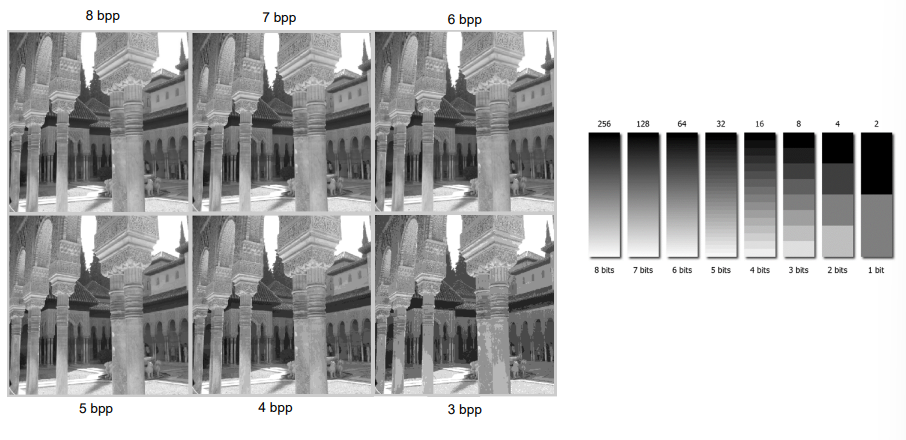
\includegraphics[width = 0.8\textwidth]{figs/profundidad.png}
\end{figure}

Aprovechando la menor sensibilidad del sistema visual humano a la información de color (crominancia) en comparación con la información de luminancia, se han desarrollado formatos que permiten comprimir imágenes reduciendo selectivamente los datos de color. Una alternativa al almacenamiento True Color (24 bpp) son las \textbf{imágenes indexadas}. En lugar de almacenar los tres valores RGB para cada píxel, se utiliza una paleta de colores o tabla de búsqueda (Color Look-Up Table - CLUT o Color Map). Esta paleta es un array de hasta 256 entradas (para 8 bpp) donde cada entrada contiene un color RGB de 24 bits.
La imagen en sí misma no almacena colores, sino índices (valores de 0 a 255) que apuntan a una posición en la paleta. Esto reduce drásticamente el tamaño del archivo. Se almacena una matriz de M×N de 8 bits (los índices) y una pequeña tabla auxiliar de 256×3 bytes (la paleta), en lugar de tres matrices de M×N de 8 bits.
No obstante, limita la imagen a un máximo de 256 colores simultáneos ($2^{nbits}$), lo que puede producir posterización (\textit{banding}) en imágenes con degradados suaves o muchas variaciones de color. Es ideal para gráficos con áreas planas de color.

\subsection{Formatos}
Hay muchos formatos de imagen:
\begin{itemize}
\item Sin compresión: BMP, RAW, PPM
\item Compresión sin pérdidas: PNG, GIF, TIFF
\item Compresión con pérdidas: JPEG, TIFF
\end{itemize}

\end{document}
